\documentclass[11pt,letterpaper]{article}

\usepackage[margin=0.78in,headheight=15pt]{geometry}
\usepackage[T1]{fontenc}
\usepackage{lmodern}
\usepackage{microtype}
\usepackage{graphicx}
\usepackage{booktabs}
\usepackage{tabularx}
\usepackage{array}
\usepackage{multirow}
\usepackage{amsmath}
\usepackage{enumitem}
\usepackage{caption}
\usepackage{subcaption}
\usepackage{float}
\usepackage{fancyhdr}
\usepackage{xcolor}
\usepackage{tikz}
\usetikzlibrary{arrows.meta,positioning,shapes.geometric,fit,calc}
\usepackage{pgfplots}
\pgfplotsset{compat=1.18}
\usepackage[most]{tcolorbox}
\usepackage{hyperref}

\definecolor{ev6navy}{HTML}{17365D}
\definecolor{ev6blue}{HTML}{2F5597}
\definecolor{ev6cyan}{HTML}{2CA6A4}
\definecolor{ev6orange}{HTML}{E07A2F}
\definecolor{ev6gold}{HTML}{D9A21B}
\definecolor{ev6green}{HTML}{3B8C5A}
\definecolor{ev6red}{HTML}{B64A4A}
\definecolor{ev6pale}{HTML}{EAF2F8}
\definecolor{ev6gray}{HTML}{5B6573}
\definecolor{ev6light}{HTML}{F4F6F8}

\hypersetup{
  colorlinks=true,
  linkcolor=ev6blue,
  urlcolor=ev6blue,
  citecolor=ev6blue,
  pdftitle={2023 Kia EV6 Wind AWD Simulink Model Calibration and Validation},
  pdfauthor={Sam Lim}
}

\pagestyle{fancy}
\fancyhf{}
\lhead{2023 Kia EV6 Wind AWD}
\rhead{Model Calibration and Validation}
\cfoot{\thepage}
\renewcommand{\headrulewidth}{0.35pt}

\setlength{\parindent}{0pt}
\setlength{\parskip}{5.5pt}
\setlist[itemize]{leftmargin=1.3em,itemsep=2pt,topsep=3pt}
\setlist[enumerate]{leftmargin=1.5em,itemsep=2pt,topsep=3pt}
\captionsetup{font=small,labelfont=bf}
\newcommand{\SI}[2]{#1\,#2}
\newcommand{\si}[1]{\mathrm{#1}}
\newcommand{\ohm}{\ensuremath{\Omega}}
\newcommand{\percent}{\%}

\newcolumntype{Y}{>{\raggedright\arraybackslash}X}
\newcolumntype{C}{>{\centering\arraybackslash}X}
\newcommand{\modelname}{\texttt{EV6\_\allowbreak LUT\_\allowbreak FourWheel\_\allowbreak EV6Battery77p4kWh\_\allowbreak PowerCorrected}}

\newtcolorbox{keybox}[1][]{
  colback=ev6pale,colframe=ev6blue,boxrule=0.6pt,arc=2pt,
  left=7pt,right=7pt,top=6pt,bottom=6pt,#1
}
\newtcolorbox{decisionbox}[1][]{
  colback=ev6light,colframe=ev6gray,boxrule=0.5pt,arc=2pt,
  left=7pt,right=7pt,top=6pt,bottom=6pt,#1
}

\tikzset{
  flow/.style={draw=ev6blue,fill=ev6pale,rounded corners=2pt,
    minimum height=9mm,text width=28mm,align=center,font=\small},
  flowdark/.style={draw=ev6navy,fill=ev6navy,text=white,rounded corners=2pt,
    minimum height=9mm,text width=28mm,align=center,font=\small\bfseries},
  decision/.style={diamond,draw=ev6orange,fill=orange!9,aspect=2.2,
    align=center,font=\footnotesize,text width=22mm},
  signal/.style={draw=ev6cyan,fill=cyan!6,rounded corners=2pt,
    minimum height=8mm,text width=28mm,align=center,font=\small},
  line/.style={-{Latex[length=2.2mm]},thick,draw=ev6gray},
  dashedline/.style={-{Latex[length=2.2mm]},thick,dashed,draw=ev6orange}
}

\begin{document}

\begin{titlepage}
  \centering
  \vspace*{0.65in}
  {\color{ev6navy}\rule{\textwidth}{2.2pt}}\\[0.35in]
  {\Huge\bfseries 2023 Kia EV6 Wind AWD\\[0.12in]
  Simulink Model Calibration and Validation\par}
  \vspace{0.28in}
  {\Large Torque Distribution, Battery Architecture, and Energy Prediction\par}
  \vspace{0.32in}
  {\color{ev6navy}\rule{0.72\textwidth}{0.8pt}}\\[0.42in]

  \begin{keybox}[width=0.86\textwidth]
  \centering
  A documented progression from a supplied Mach-E-based model to an
  EV6-specific longitudinal model using measured chassis-dynamometer data,
  training/validation separation, least-squares identification, and a
  speed/mode-dependent battery-power correction.
  \end{keybox}

  \vfill
  \begin{tabular}{rl}
    \textbf{Prepared by:} & Sam Lim \\
    \textbf{Laboratory:} & UGA Mobility Systems Controls Laboratory \\
    \textbf{Prepared for:} & Dr. Yunli Shao \\
    \textbf{Vehicle:} & 2023 Kia EV6 Wind AWD, Dual Motor \\
    \textbf{Date:} & September 28, 2026
  \end{tabular}
  \vfill
  {\color{ev6navy}\rule{\textwidth}{2.2pt}}
\end{titlepage}

\pagenumbering{roman}
\tableofcontents
\clearpage
\pagenumbering{arabic}

\section{Executive Summary}

This work converted a supplied 2024a Mach-E-based Simulink vehicle model into a
calibrated model of a 2023 Kia EV6 Wind AWD. The development used four EV6
chassis-dynamometer runs sampled at approximately \SI{1}{ms}. Runs 001--003
were used for parameter identification and map development; Run 004 was used as
a development-validation cycle and for final model evaluation.

The work proceeded in stages. First, the external speed input was corrected so
the model followed the same cycle as the dyno vehicle. Next, a three-dimensional
front/rear torque-distribution lookup table and two torque gains were introduced.
The original battery configuration was then replaced by an equivalent
\SI{77.4}{kWh}, \SI{697}{V} EV6 battery representation. Finally, a
speed- and operating-mode-dependent power correction was added at the battery
current summation point. The correction improved electrical and energy
prediction without changing the mechanical response of the vehicle.

\begin{keybox}
\textbf{Final result on Run 004:} the net-energy error decreased from
\SI{-22.965}{\percent} to \SI{-1.808}{\percent}; battery-current MAE decreased
from \SI{1.222}{A} to \SI{0.971}{A}; and the corrected current correlation was
0.9784. Vehicle speed and wheel torque were preserved to effective numerical
precision.
\end{keybox}

\begin{figure}[H]
\centering
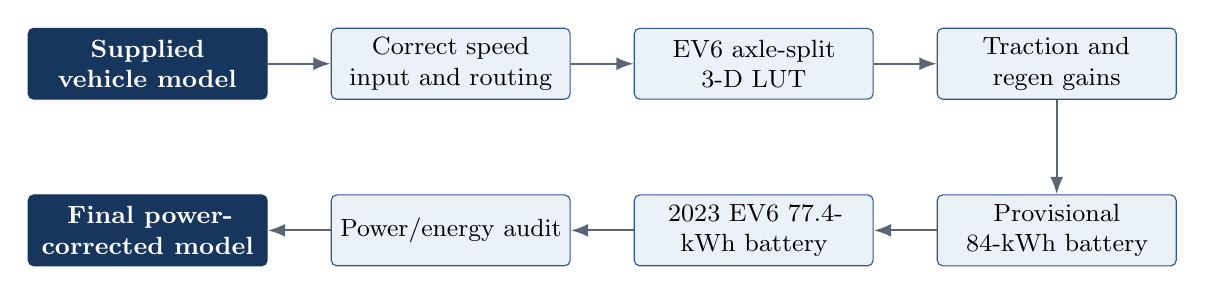
\begin{tikzpicture}[node distance=8mm and 8mm]
  \node[flowdark] (base) {Supplied vehicle model};
  \node[flow,right=of base] (input) {Correct speed input and routing};
  \node[flow,right=of input] (lut) {EV6 axle-split 3-D LUT};
  \node[flow,right=of lut] (gains) {Traction and regen gains};

  \node[flow,below=12mm of gains] (b84) {Provisional 84-kWh battery};
  \node[flow,left=of b84] (b77) {2023 EV6 77.4-kWh battery};
  \node[flow,left=of b77] (audit) {Power/energy audit};
  \node[flowdark,left=of audit] (final) {Final power-corrected model};

  \draw[line] (base)--(input);
  \draw[line] (input)--(lut);
  \draw[line] (lut)--(gains);
  \draw[line] (gains)--(b84);
  \draw[line] (b84)--(b77);
  \draw[line] (b77)--(audit);
  \draw[line] (audit)--(final);
\end{tikzpicture}
\caption{Model-development sequence. Each step was retained only after a targeted diagnostic or validation check.}
\end{figure}

\section{Scope, Data, and Experimental Strategy}

\subsection{Vehicle definition}

The confirmed test vehicle was a 2023 Kia EV6 Wind AWD with dual motors. The
official specification sheet was used to anchor the high-level physical model:
\SI{77.4}{kWh} battery energy, \SI{697}{V} nominal pack voltage, AWD dual-motor
architecture, and a 10.65:1 final-drive ratio \cite{kia2023}. The internal
series/parallel battery topology used here is an \emph{equivalent model
topology}; it is not a claim about the production cell arrangement.

\subsection{Dyno runs}

\begin{table}[H]
\centering
\caption{Measured drive-cycle datasets.}
\begin{tabular}{lrrrr}
\toprule
Run & Samples & Duration (s) & Current range (A) & Voltage range (V) \\
\midrule
001 & 1,433,737 & 1,433.793 & $-45.8$ to $63.8$ & 725.6 to 741.3 \\
002 & 1,428,146 & 1,428.202 & $-41.3$ to $66.2$ & 722.1 to 737.2 \\
003 & 621,577   & 621.601   & $-38.6$ to $48.0$ & 720.6 to 730.8 \\
004 & 619,377   & 619.401   & $-35.5$ to $43.7$ & 720.3 to 729.5 \\
\bottomrule
\end{tabular}
\end{table}

\begin{figure}[H]
\centering
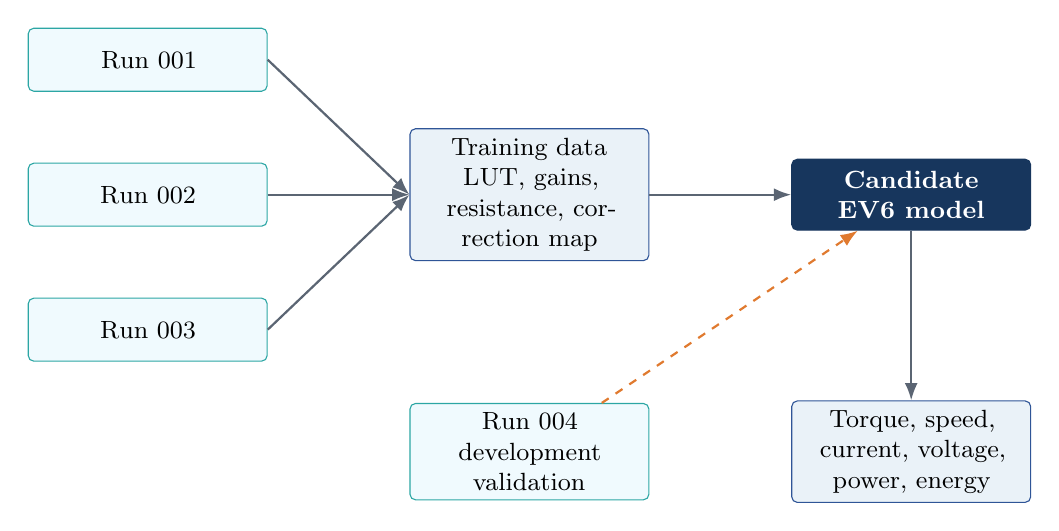
\begin{tikzpicture}[node distance=9mm and 10mm]
  \node[signal] (r1) {Run 001};
  \node[signal,below=of r1] (r2) {Run 002};
  \node[signal,below=of r2] (r3) {Run 003};
  \node[flow,right=18mm of r2] (train) {Training data\\LUT, gains, resistance, correction map};
  \node[flowdark,right=18mm of train] (cand) {Candidate EV6 model};
  \node[signal,below=18mm of train] (r4) {Run 004\\development validation};
  \node[flow,right=18mm of r4] (metrics) {Torque, speed, current, voltage, power, energy};
  \draw[line] (r1.east)--(train.west);
  \draw[line] (r2.east)--(train.west);
  \draw[line] (r3.east)--(train.west);
  \draw[line] (train)--(cand);
  \draw[dashedline] (r4)--(cand);
  \draw[line] (cand)--(metrics);
\end{tikzpicture}
\caption{Identification and validation workflow. Run 004 was not used in the initial least-squares training, but it was later used to select the 0.50 correction-map scale; it is therefore a development-validation cycle rather than a completely untouched test set.}
\end{figure}

\section{Development and Decision Process}

\subsection{Stage 1: Preserve the Supplied Baseline}

The supplied model was retained unchanged. A separate working copy was created
for every major branch: true pre-LUT baseline, LUT-only, LUT plus gains,
provisional battery candidates, and the final power-corrected model. This made
the effect of each change measurable and prevented the original asset from
being overwritten.

\subsection{Stage 2: Correct the Speed-demand Source}

The first battery comparison was invalid because the simulation did not use the
Run 004 speed trace. During an early 5--60 second check, the simulation
reference reached \SI{21.279}{m/s}, while the dyno speed reached only
\SI{7.759}{m/s}. The resulting speed RMSE was \SI{12.273}{m/s}; current and
voltage differences from that run were consequences of mismatched vehicle
demand, not battery calibration.

Tracing all \texttt{From Workspace} blocks showed that the active top-level
speed source was different from the assumed internal compatibility signal. The
Run 004 signal was then assigned to the active source. The corrected reference
matched the dyno exactly in the short diagnostic (RMSE \SI{0}{m/s}, correlation
1.000000), while actual speed had RMSE \SI{0.215}{m/s} and correlation 0.999891.

\begin{decisionbox}
\textbf{Decision rule:} no battery or powertrain parameter was accepted from a
simulation until the reference-speed trace matched the dyno cycle. This avoided
calibrating physical parameters to compensate for an input-routing error.
\end{decisionbox}

\subsection{Stage 3: Establish a True pre-LUT Baseline}

The initial baseline copy produced zero motor command because its manual/auto
routing selected inactive external pedal channels. The routing was traced from
the subsystem inports through the auto-pilot switches. After the active driver
path was restored, the true pre-LUT model completed Run 004 and established a
valid comparison point. Its four-wheel torque MAE was \SI{152.23}{N.m}, torque
RMSE was \SI{252.63}{N.m}, and speed RMSE was \SI{1.2511}{m/s}.

\subsection{Stage 4: Add EV6 Torque Distribution and Gains}

A three-dimensional lookup table distributed total signed axle torque between
the front and rear axles. The LUT was trained from Runs 001--003 and indexed by
vehicle speed, longitudinal acceleration, and signed total axle torque. Separate
traction and regeneration gains were applied after the split was established.

\begin{figure}[H]
\centering
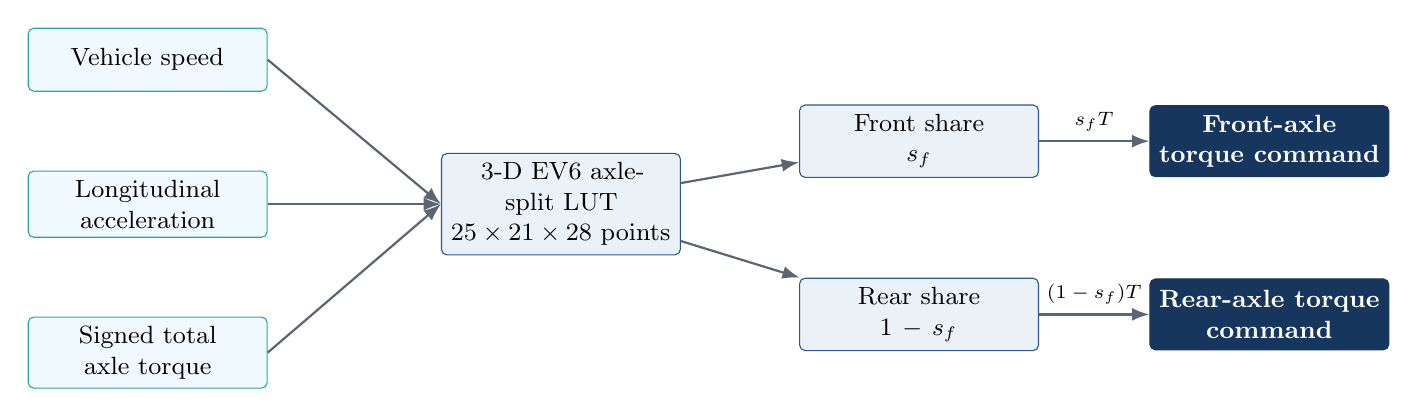
\begin{tikzpicture}[node distance=10mm and 11mm]
  \node[signal] (spd) {Vehicle speed};
  \node[signal,below=of spd] (acc) {Longitudinal acceleration};
  \node[signal,below=of acc] (trq) {Signed total axle torque};
  \node[flow,right=22mm of acc] (lut) {3-D EV6 axle-split LUT\\$25\times21\times28$ points};
  \node[flow,right=15mm of lut,yshift=8mm] (front) {Front share\\$s_f$};
  \node[flow,right=15mm of lut,yshift=-14mm] (rear) {Rear share\\$1-s_f$};
  \node[flowdark,right=14mm of front] (fcmd) {Front-axle torque command};
  \node[flowdark,right=14mm of rear] (rcmd) {Rear-axle torque command};
  \draw[line] (spd.east)--(lut.west);
  \draw[line] (acc.east)--(lut.west);
  \draw[line] (trq.east)--(lut.west);
  \draw[line] (lut)--(front);
  \draw[line] (lut)--(rear);
  \draw[line] (front)--node[above,font=\scriptsize]{$s_f T$}(fcmd);
  \draw[line] (rear)--node[above,font=\scriptsize]{$(1-s_f)T$}(rcmd);
\end{tikzpicture}
\caption{EV6 torque-distribution model. The LUT contains 14,700 operating points and covers traction (0 to \SI{1300}{N.m}) and regeneration (\SI{-1400}{N.m} to 0).}
\end{figure}

The selected gains were 1.223989 for traction torque and 1.348705 for
regeneration torque. Relative to the true pre-LUT baseline, the LUT alone
reduced four-wheel torque MAE by 36.97\%. The gains provided a smaller but
consistent additional improvement, reaching a total MAE reduction of 39.98\%.

\subsection{Stage 5: Diagnose the Battery Architecture}

The original pack model used 96 series cells and three parallel branches, a
\SI{60}{Ah} branch capacity, and initial SOC 0.90. At that SOC, its open-circuit
voltage table predicted a pack voltage of approximately \SI{390.8}{V}, while
the dyno pack was near \SI{726}{V}. The voltage ratio of 1.858 immediately
showed that resistance tuning alone could not correct the battery model.

A provisional 84-kWh, 192s2p model was used to verify the architecture and
signal path. After the exact vehicle trim was confirmed, it was replaced by the
final 77.4-kWh equivalent pack. This avoided preserving a temporary assumption
after an official specification became available.

\begin{table}[H]
\centering
\caption{Battery architecture progression.}
\begin{tabularx}{\textwidth}{Yrrrrr}
\toprule
Model stage & Series & Parallel & Pack capacity (Ah) & Initial SOC & Initial OCV (V) \\
\midrule
Original supplied battery & 96 & 3 & 180.000 & 0.9000 & 390.817 \\
Provisional 84-kWh candidate & 192 & 2 & 120.600 & 0.6389 & 726.472 \\
Final 2023 EV6 equivalent & 192 & 2 & 111.047 & 0.638879 & 726.472 \\
\bottomrule
\end{tabularx}
\end{table}

Least-squares identification from Runs 001--003 estimated a common pack
resistance of \SI{0.132764}{\ohm}. The original model produced approximately
\SI{0.027992}{\ohm} at \SI{298.1}{K} and 90\% SOC. A resistance-table scale of
1.84965 was therefore applied in the final EV6 battery candidate. The
identified resistance is an effective model value that captures terminal
voltage behavior; it should not be interpreted as a direct laboratory DCIR
measurement.

\section{Power and Energy Correction}

\subsection{Energy calculation audit}

Because current and voltage appeared visually close while cumulative energy did
not, the energy calculation was audited before any further tuning. All four
methods---direct \texttt{trapz}, explicit trapezoids, \texttt{cumtrapz}
endpoint, and positive energy minus regenerative energy---returned the same
dyno value of \SI{0.28431}{kWh} on Run 004. The sign convention was also checked
against the direct Simulink battery-power signal.

\begin{align}
P_{\mathrm{batt}}(t) &= \frac{V_{\mathrm{pack}}(t) I_{\mathrm{pack}}(t)}{1000}
\quad [\si{kW}], \\
E_{\mathrm{net}} &= \frac{1}{3600}\int_{t_0}^{t_f}P_{\mathrm{batt}}(t)\,dt
\quad [\si{kWh}].
\end{align}

The original Run 004 power bias was \SI{-0.3826}{kW} over 0.17067 hours. Its
predicted energy difference, \SI{-0.06530}{kWh}, exactly matched the measured
energy deficit. This confirmed that the discrepancy was a sustained power bias,
not an integration bug.

\subsection{Stationary auxiliary load}

At vehicle standstill, the dyno vehicle consistently consumed about
\SI{0.364}{kW}, while the original simulation consumed approximately zero.
This is physically plausible for HVAC, infotainment, control computers, pumps,
and other auxiliary systems. A training-only stationary estimate gave
\SI{0.3643}{kW}, equivalent to roughly \SI{0.499}{A} at the EV6 pack voltage.

\begin{figure}[H]
\centering
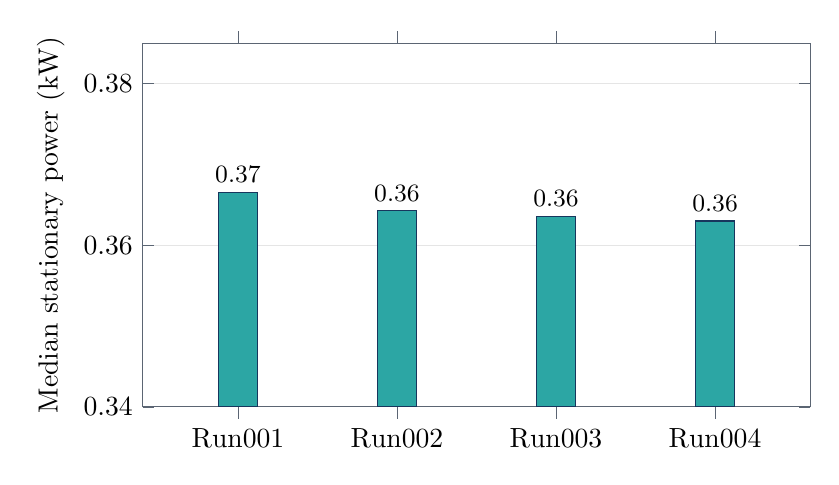
\begin{tikzpicture}
\begin{axis}[
  ybar,bar width=14pt,width=0.83\textwidth,height=6.2cm,
  ymin=0.34,ymax=0.385,
  ylabel={Median stationary power (kW)},
  symbolic x coords={Run001,Run002,Run003,Run004},xtick=data,
  nodes near coords,nodes near coords align={vertical},
  every node near coord/.append style={font=\small},
  axis line style={draw=ev6gray},tick style={draw=ev6gray},
  ymajorgrids=true,grid style={draw=gray!20},
  enlarge x limits=0.20]
\addplot[fill=ev6cyan,draw=ev6navy] coordinates {
  (Run001,0.36655) (Run002,0.36425) (Run003,0.36360) (Run004,0.36300)};
\end{axis}
\end{tikzpicture}
\caption{Measured median battery power during stationary dwell. The narrow spread supports a nearly fixed auxiliary-load component.}
\end{figure}

A separate constant auxiliary block was tested offline but not retained in the
final model. The existing speed/mode correction already captured part of the
stationary load, so adding both terms would double-count that energy. This is
an important modeling decision: the \SI{0.3643}{kW} estimate remains a useful
physical interpretation, but the final implementation uses one correction path.

\subsection{Speed/mode correction map}

Residual power error was separated into traction, regeneration, and low-power
operating modes using a \SI{0.5}{kW} mode threshold. For each mode, the mean
required correction was estimated in nine speed bins from Runs 001--003,
smoothed, and multiplied by a conservative map scale of 0.50. The map scale was
selected because the unscaled candidate over-corrected Run 004 energy.

\begin{figure}[H]
\centering
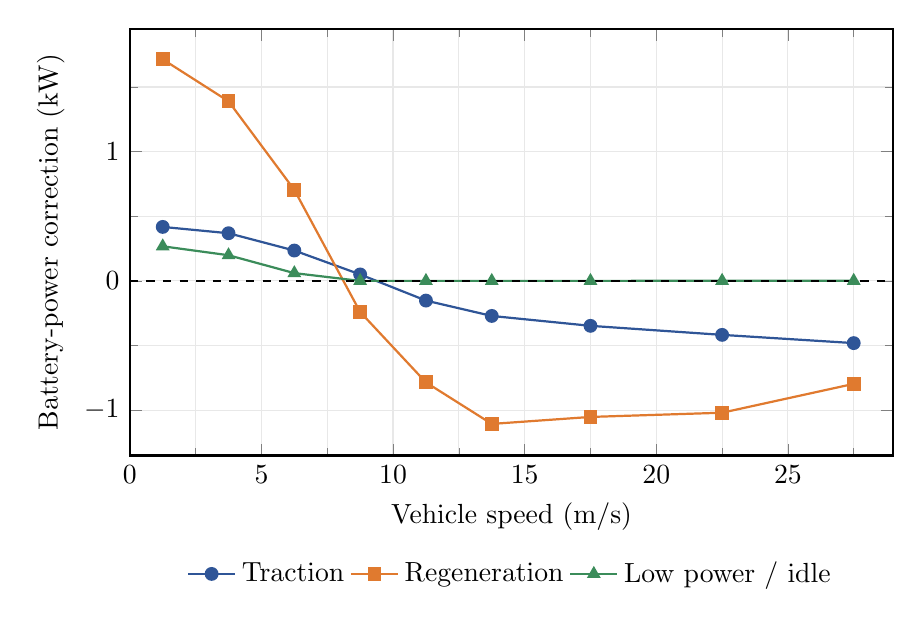
\begin{tikzpicture}
\begin{axis}[
  width=0.93\textwidth,height=7.0cm,
  xlabel={Vehicle speed (m/s)},ylabel={Battery-power correction (kW)},
  xmin=0,xmax=29,ymin=-1.35,ymax=1.95,
  grid=both,minor tick num=1,grid style={draw=gray!18},
  legend style={at={(0.5,-0.22)},anchor=north,legend columns=3,draw=none},
  thick,mark size=2.1pt]
\addplot[color=ev6blue,mark=*] coordinates {
 (1.25,0.41746) (3.75,0.36861) (6.25,0.23472) (8.75,0.049994)
 (11.25,-0.15238) (13.75,-0.27109) (17.5,-0.34766)
 (22.5,-0.41754) (27.5,-0.48122)};
\addlegendentry{Traction}
\addplot[color=ev6orange,mark=square*] coordinates {
 (1.25,1.7139) (3.75,1.3892) (6.25,0.70382) (8.75,-0.24035)
 (11.25,-0.78513) (13.75,-1.1063) (17.5,-1.0523)
 (22.5,-1.0197) (27.5,-0.79652)};
\addlegendentry{Regeneration}
\addplot[color=ev6green,mark=triangle*] coordinates {
 (1.25,0.26762) (3.75,0.19843) (6.25,0.06005) (8.75,0)
 (11.25,0) (13.75,0) (17.5,0) (22.5,0.00078059) (27.5,0.00078059)};
\addlegendentry{Low power / idle}
\addplot[black,dashed,domain=0:29,samples=2] {0};
\end{axis}
\end{tikzpicture}
\caption{Final 0.50-scaled speed/mode battery-power correction map. Positive values increase battery power draw; negative values reduce it.}
\end{figure}

\begin{table}[H]
\centering
\caption{Numerical correction map implemented in the candidate.}
\small
\begin{tabular}{rrrr}
\toprule
Speed (m/s) & Traction (kW) & Regeneration (kW) & Low power (kW) \\
\midrule
1.25  &  0.4175 &  1.7139 & 0.2676 \\
3.75  &  0.3686 &  1.3892 & 0.1984 \\
6.25  &  0.2347 &  0.7038 & 0.0601 \\
8.75  &  0.0500 & $-0.2403$ & 0.0000 \\
11.25 & $-0.1524$ & $-0.7851$ & 0.0000 \\
13.75 & $-0.2711$ & $-1.1063$ & 0.0000 \\
17.50 & $-0.3477$ & $-1.0523$ & 0.0000 \\
22.50 & $-0.4175$ & $-1.0197$ & 0.0008 \\
27.50 & $-0.4812$ & $-0.7965$ & 0.0008 \\
\bottomrule
\end{tabular}
\end{table}

\subsection{Physical implementation in Simulink}

The map output is a battery-power correction. It is converted to a current
correction using pack voltage and injected at the existing battery-current sum.
This placement changes battery terminal current, voltage, power, SOC, and energy
consistently, while leaving the requested motor torque and vehicle dynamics
unchanged.

\begin{figure}[H]
\centering
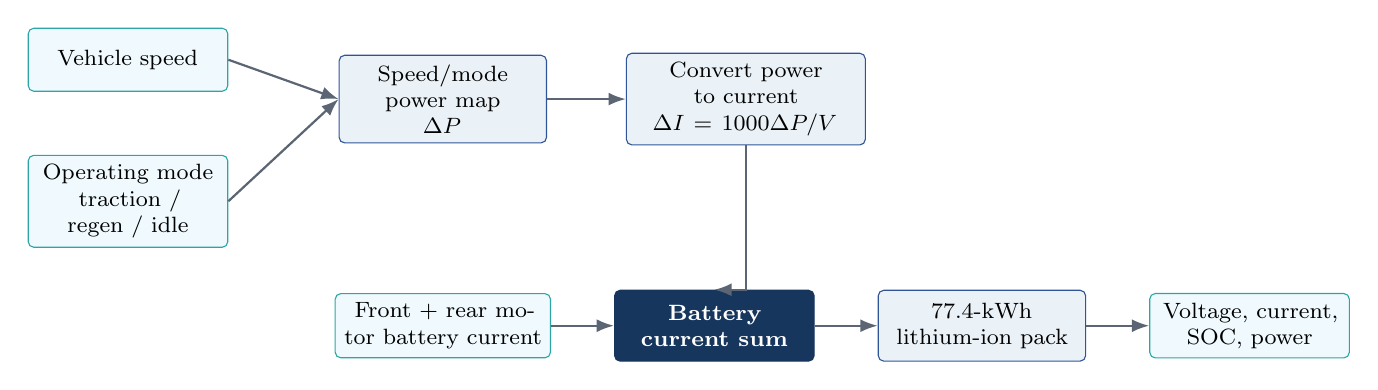
\begin{tikzpicture}[node distance=8mm and 8mm]
  \node[signal,text width=23mm,font=\footnotesize] (speed) {Vehicle speed};
  \node[signal,text width=23mm,font=\footnotesize,below=of speed] (mode) {Operating mode\\traction / regen / idle};
  \node[flow,text width=24mm,font=\footnotesize,right=14mm of speed,yshift=-5mm] (map) {Speed/mode power map\\$\Delta P$};
  \node[flow,text width=28mm,font=\footnotesize,right=10mm of map] (convert) {Convert power to current\\$\Delta I=1000\Delta P/V$};
  \node[signal,text width=25mm,font=\footnotesize,below=19mm of map] (base) {Front + rear motor battery current};
  \node[flowdark,text width=23mm,font=\footnotesize\bfseries,right=8mm of base] (sum) {Battery current sum};
  \node[flow,text width=24mm,font=\footnotesize,right=8mm of sum] (pack) {77.4-kWh lithium-ion pack};
  \node[signal,text width=23mm,font=\footnotesize,right=8mm of pack] (out) {Voltage, current, SOC, power};
  \draw[line] (speed.east)--(map.west);
  \draw[line] (mode.east)--(map.west);
  \draw[line] (map)--(convert);
  \draw[line] (convert.south)|-(sum.north);
  \draw[line] (base)--(sum);
  \draw[line] (sum)--(pack);
  \draw[line] (pack)--(out);
\end{tikzpicture}
\caption{Battery-current correction signal path in the final Simulink model.}
\end{figure}

\section{Final Validation Results}

\subsection{Mechanical performance}

\begin{figure}[H]
\centering
\begin{subfigure}[t]{0.49\textwidth}
\centering
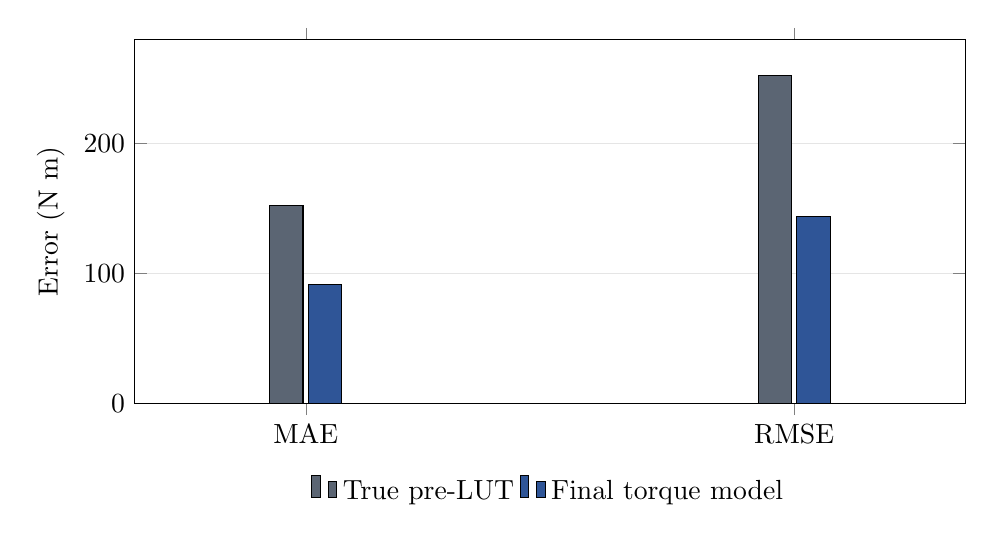
\begin{tikzpicture}
\begin{axis}[
  ybar,bar width=12pt,width=\textwidth,height=6.2cm,
  ylabel={Error (N m)},symbolic x coords={MAE,RMSE},xtick=data,
  ymin=0,ymax=280,legend style={at={(0.5,-0.18)},anchor=north,legend columns=2,draw=none},
  ymajorgrids=true,grid style={draw=gray!20},enlarge x limits=0.35]
\addplot[fill=ev6gray] coordinates {(MAE,152.23) (RMSE,252.63)};
\addlegendentry{True pre-LUT}
\addplot[fill=ev6blue] coordinates {(MAE,91.373) (RMSE,143.79)};
\addlegendentry{Final torque model}
\end{axis}
\end{tikzpicture}
\caption{Four-wheel torque error.}
\end{subfigure}
\hfill
\begin{subfigure}[t]{0.49\textwidth}
\centering
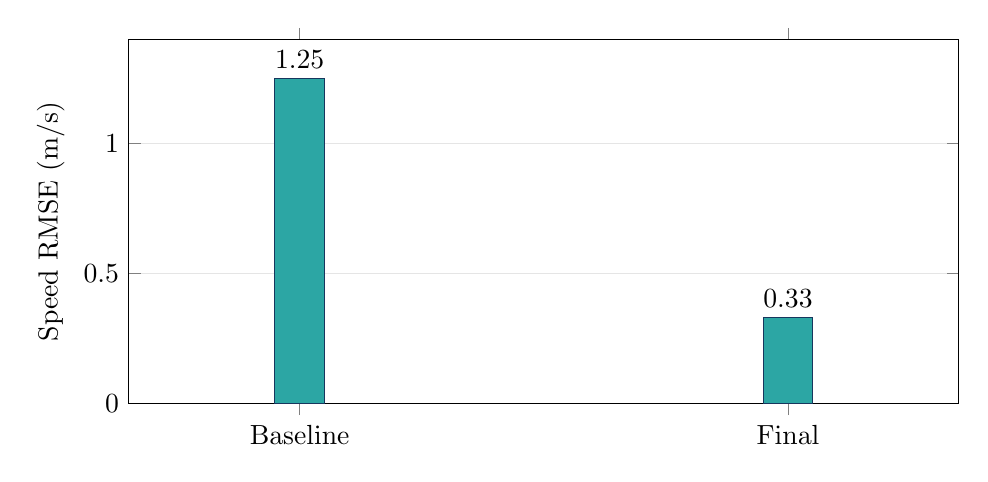
\begin{tikzpicture}
\begin{axis}[
  ybar,bar width=18pt,width=\textwidth,height=6.2cm,
  ylabel={Speed RMSE (m/s)},symbolic x coords={Baseline,Final},xtick=data,
  ymin=0,ymax=1.4,nodes near coords,nodes near coords align={vertical},
  ymajorgrids=true,grid style={draw=gray!20},enlarge x limits=0.35]
\addplot[fill=ev6cyan,draw=ev6navy] coordinates {(Baseline,1.2511) (Final,0.33211)};
\end{axis}
\end{tikzpicture}
\caption{Vehicle-speed tracking.}
\end{subfigure}
\caption{Mechanical improvements from the supplied baseline to the final calibrated torque model.}
\end{figure}

The final torque model reduced four-wheel MAE by 39.98\% and RMSE by 43.08\%.
Vehicle-speed RMSE decreased by 73.46\%. These improvements occurred before the
battery power correction was applied.

\subsection{Electrical performance}

\begin{table}[H]
\centering
\caption{Full Run 004 electrical metrics, 5.0--619.4 seconds.}
\begin{tabular}{llrrrr}
\toprule
Signal & Model & Bias & MAE & RMSE & Correlation \\
\midrule
Current (A) & Original 77.4-kWh & $-0.5242$ & 1.2219 & 2.1174 & 0.9740 \\
Current (A) & Power corrected & $-0.0387$ & 0.9713 & 1.8678 & 0.9784 \\
Voltage (V) & Original 77.4-kWh & $-0.2797$ & 0.6586 & 1.5988 & 0.6521 \\
Voltage (V) & Power corrected & 0.0145 & 0.2690 & 0.4150 & 0.9560 \\
Power (kW) & Original 77.4-kWh & $-0.3826$ & 0.8880 & 1.5419 & 0.9738 \\
Power (kW) & Power corrected & $-0.0301$ & 0.7058 & 1.3598 & 0.9782 \\
\bottomrule
\end{tabular}
\end{table}

\begin{figure}[H]
\centering
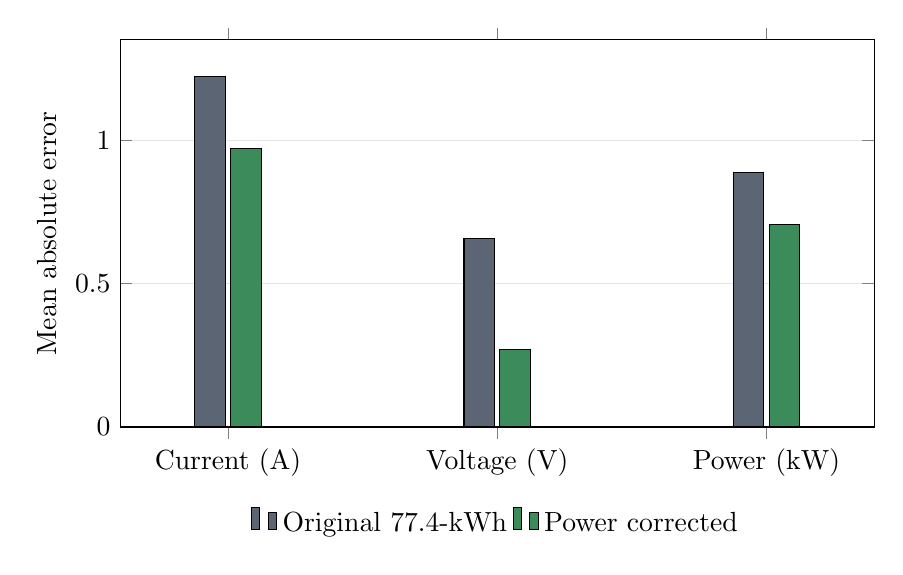
\begin{tikzpicture}
\begin{axis}[
  ybar,bar width=11pt,width=0.92\textwidth,height=6.5cm,
  ylabel={Mean absolute error},
  symbolic x coords={Current (A),Voltage (V),Power (kW)},xtick=data,
  ymin=0,ymax=1.35,
  legend style={at={(0.5,-0.19)},anchor=north,legend columns=2,draw=none},
  ymajorgrids=true,grid style={draw=gray!20},enlarge x limits=0.20]
\addplot[fill=ev6gray] coordinates {(Current (A),1.2219) (Voltage (V),0.65858) (Power (kW),0.88796)};
\addlegendentry{Original 77.4-kWh}
\addplot[fill=ev6green] coordinates {(Current (A),0.97128) (Voltage (V),0.26896) (Power (kW),0.70579)};
\addlegendentry{Power corrected}
\end{axis}
\end{tikzpicture}
\caption{Electrical mean-absolute-error comparison on the full Run 004 cycle.}
\end{figure}

The battery-current result is the primary electrical validation because EV
pack voltage is comparatively constant. The corrected model follows the
measured current shape with correlation 0.9784 and reduces current MAE by
20.51\%. Voltage agreement also improves, but voltage alone is not sufficient
to demonstrate accurate energy prediction.

\subsection{Energy performance}

\begin{figure}[H]
\centering
\begin{subfigure}[t]{0.50\textwidth}
\centering
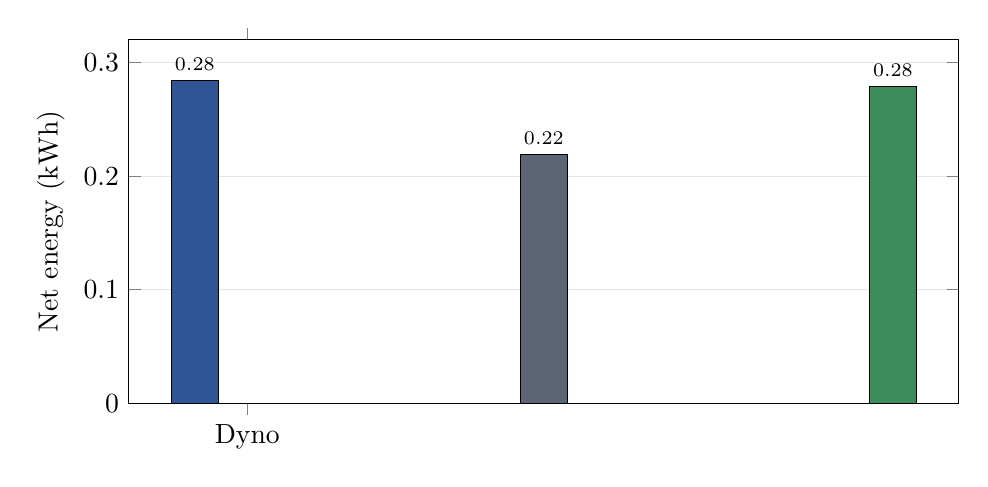
\begin{tikzpicture}
\begin{axis}[
  ybar,bar width=17pt,width=\textwidth,height=6.2cm,
  ylabel={Net energy (kWh)},
  symbolic x coords={Dyno,Original,Final},xtick=data,
  ymin=0,ymax=0.32,nodes near coords,nodes near coords align={vertical},
  every node near coord/.append style={font=\scriptsize},
  ymajorgrids=true,grid style={draw=gray!20},enlarge x limits=0.20]
\addplot[fill=ev6blue] coordinates {(Dyno,0.28431)};
\addplot[fill=ev6gray] coordinates {(Original,0.21902)};
\addplot[fill=ev6green] coordinates {(Final,0.27917)};
\end{axis}
\end{tikzpicture}
\caption{Integrated net energy.}
\end{subfigure}
\hfill
\begin{subfigure}[t]{0.46\textwidth}
\centering
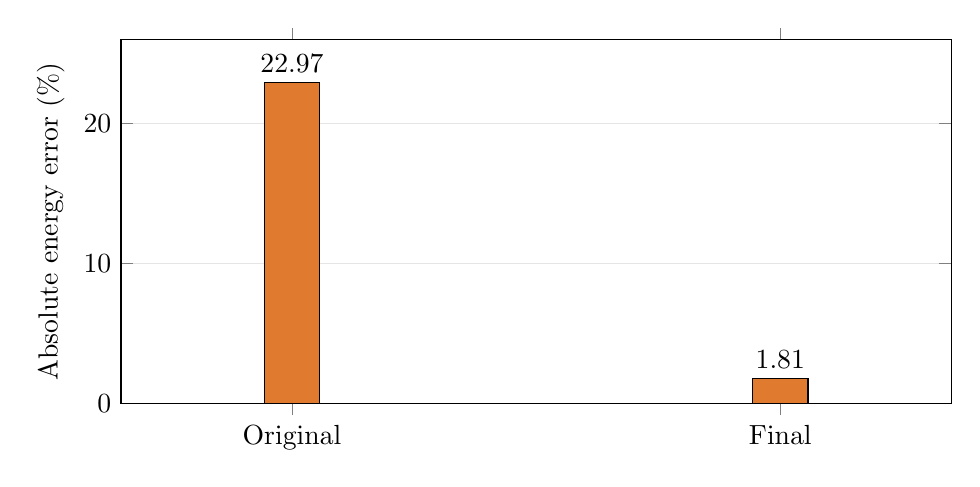
\begin{tikzpicture}
\begin{axis}[
  ybar,bar width=20pt,width=\textwidth,height=6.2cm,
  ylabel={Absolute energy error (\%)},
  symbolic x coords={Original,Final},xtick=data,
  ymin=0,ymax=26,nodes near coords,nodes near coords align={vertical},
  ymajorgrids=true,grid style={draw=gray!20},enlarge x limits=0.35]
\addplot[fill=ev6orange] coordinates {(Original,22.965) (Final,1.8076)};
\end{axis}
\end{tikzpicture}
\caption{Absolute net-energy error.}
\end{subfigure}
\caption{Full-cycle energy validation. The final model is \SI{5.139}{Wh} below the dyno result.}
\end{figure}

\begin{table}[H]
\centering
\caption{Full-cycle energy decomposition.}
\begin{tabular}{lrrr}
\toprule
Dataset & Net energy (kWh) & Positive energy (kWh) & Regen magnitude (kWh) \\
\midrule
EV6 dyno & 0.28431 & 0.46074 & 0.17643 \\
Original 77.4-kWh model & 0.21902 & 0.41266 & 0.19364 \\
Power-corrected model & 0.27917 & 0.44817 & 0.16899 \\
\bottomrule
\end{tabular}
\end{table}

The final model reduced the absolute net-energy error by 21.16 percentage
points, or 92.13\% relative to the original error. Positive-energy error was
\SI{-2.73}{\percent}, and regenerative-energy error was \SI{-4.21}{\percent}.

\subsection{Dynamics-preservation check}

The battery correction must not improve energy by changing requested vehicle
motion. A direct comparison of the original 77.4-kWh model and the
power-corrected model showed a speed RMSE difference of only
\SI{4.975e-5}{m/s} and a four-wheel torque RMSE difference of
\SI{0.1665}{N.m}. Both correlations were effectively 1.0.

\begin{figure}[H]
\centering
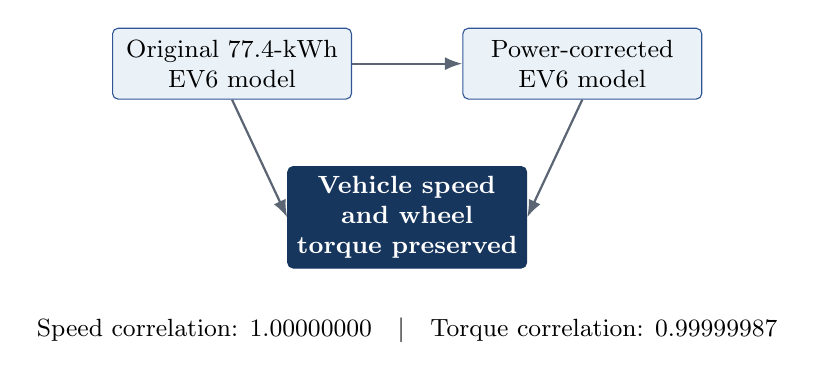
\begin{tikzpicture}[node distance=12mm and 14mm]
  \node[flow] (original) {Original 77.4-kWh EV6 model};
  \node[flow] (corrected) [right=of original] {Power-corrected EV6 model};
  \node[flowdark] (motion) [below=13mm of $(original)!0.5!(corrected)$] {Vehicle speed and wheel torque preserved};
  \draw[line] (original)--(corrected);
  \draw[line] (original.south)--(motion.west);
  \draw[line] (corrected.south)--(motion.east);
  \node[below=5mm of motion,font=\small,align=center] {Speed correlation: 1.00000000\quad $\vert$\quad Torque correlation: 0.99999987};
\end{tikzpicture}
\caption{The final correction changes electrical behavior while preserving mechanical dynamics.}
\end{figure}

\section{What Changed in the Final Model}

\begin{table}[H]
\centering
\caption{Final model changes and their engineering basis.}
\begin{tabularx}{\textwidth}{p{0.23\textwidth}Y Y}
\toprule
Change & Basis & Purpose \\
\midrule
Active drive-cycle input & Trace of active \texttt{From Workspace} routing & Ensure simulation and dyno receive identical speed demand \\
3-D front/rear torque LUT & Runs 001--003 wheel-torque data & Reproduce EV6 AWD torque distribution \\
Traction and regen gains & Training-run torque calibration & Correct overall commanded torque magnitude \\
77.4-kWh, 697-V pack & Official 2023 EV6 Wind AWD specification & Match vehicle energy and voltage class \\
192s2p equivalent topology & Dyno OCV and model-table compatibility & Reproduce approximately \SI{726}{V} initial pack OCV \\
Resistance-table scale & Least-squares voltage-current fit & Match effective terminal-voltage response \\
Speed/mode power map & Residual power error from Runs 001--003 & Remove systematic energy and current bias \\
\bottomrule
\end{tabularx}
\end{table}

The original supplied model was not modified. The final working model is:
\begin{center}
\small\texttt{EV6\_LUT\_FourWheel\_EV6Battery77p4kWh\_}\allowbreak
\texttt{PowerCorrected.slx}
\end{center}
The correction-map subsystem is intentionally battery-side; it is not a new
pedal-to-current LUT and it does not alter axle torque commands.

\section{Decisions Considered but Not Retained}

\begin{table}[H]
\centering
\caption{Alternatives rejected during development.}
\begin{tabularx}{\textwidth}{p{0.24\textwidth}Y Y}
\toprule
Alternative & Why it was considered & Why it was not retained \\
\midrule
Tune battery resistance only & Initial voltage error appeared electrical & The 96-series architecture limited pack OCV to about \SI{391}{V}; topology had to be corrected first \\
Keep the 84-kWh candidate & It produced the correct voltage class and validated the signal path & Confirmed vehicle was a 2023 model with an official \SI{77.4}{kWh} pack \\
Use one global power scale & Simple least-squares fit & Error changed sign with speed and mode; one scale could not generalize \\
Use unscaled correction map & Fit training residuals more aggressively & It over-corrected Run 004; a 0.50 scale gave better balance \\
Add a separate fixed auxiliary block & Stationary data showed about \SI{0.364}{kW} load & The speed/mode map already captured part of that load, creating double counting \\
Add pedal-to-current LUT & Suggested if current remained poorly matched & Current correlation already reached 0.9784; energy bias was addressed more directly at the battery power level \\
\bottomrule
\end{tabularx}
\end{table}

\section{Final Performance Summary}

\begin{table}[H]
\centering
\caption{Primary before/after metrics.}
\begin{tabular}{lrrrr}
\toprule
Metric & Initial & Final & Unit & Improvement \\
\midrule
Four-wheel torque MAE & 152.23 & 91.373 & N m & 39.98\% \\
Four-wheel torque RMSE & 252.63 & 143.79 & N m & 43.08\% \\
Vehicle-speed RMSE & 1.2511 & 0.33211 & m/s & 73.46\% \\
Battery-current MAE & 1.2219 & 0.97128 & A & 20.51\% \\
Battery-power MAE & 0.88796 & 0.70579 & kW & 20.52\% \\
Absolute net-energy error & 22.965 & 1.8076 & \% & 92.13\% \\
\bottomrule
\end{tabular}
\end{table}

\begin{figure}[H]
\centering
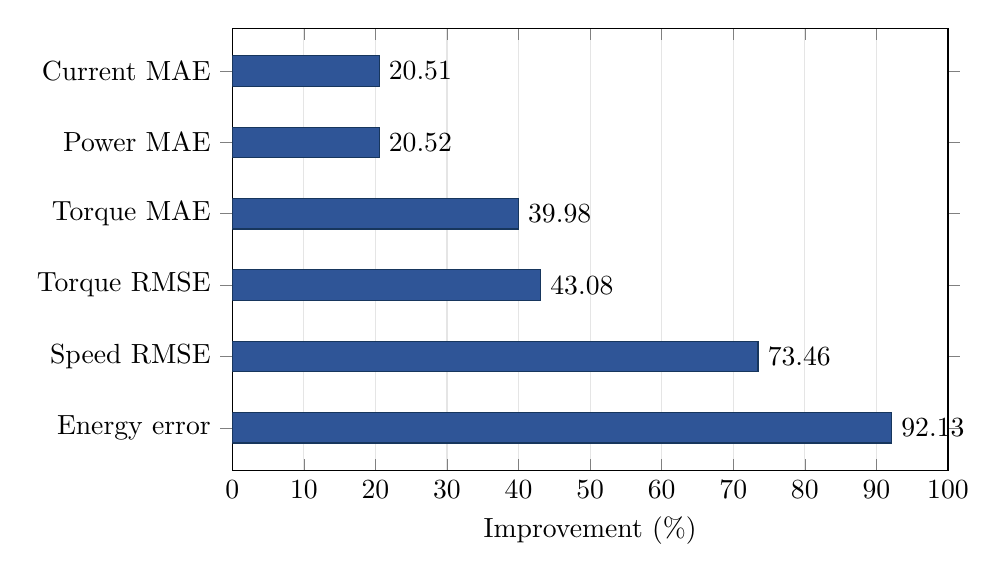
\begin{tikzpicture}
\begin{axis}[
  xbar,bar width=11pt,width=0.88\textwidth,height=7.2cm,
  xlabel={Improvement (\%)},xmin=0,xmax=100,
  symbolic y coords={Energy error,Speed RMSE,Torque RMSE,Torque MAE,Power MAE,Current MAE},
  ytick=data,nodes near coords,nodes near coords align={horizontal},
  xmajorgrids=true,grid style={draw=gray!20},
  enlarge y limits=0.12]
\addplot[fill=ev6blue,draw=ev6navy] coordinates {
 (92.129,Energy error) (73.455,Speed RMSE) (43.084,Torque RMSE)
 (39.976,Torque MAE) (20.515,Power MAE) (20.508,Current MAE)};
\end{axis}
\end{tikzpicture}
\caption{Relative improvement of the final model over the applicable baseline for each metric.}
\end{figure}

\section{Reproduction and Deliverables}

The final package was organized under
\texttt{EV6\_Final\_Package\_2023\_Wind\_AWD}. The minimum files required to
reproduce the desktop simulation are:

\begin{itemize}
  \item \texttt{EV6\_LUT\_FourWheel\_EV6Battery77p4kWh\_PowerCorrected.slx};
  \item \texttt{init\_EV6\_model.m};
  \item \texttt{EV6\_axle\_split\_LUT\_3D.mat};
  \item \texttt{EV6\_CombinedTrainingCalibration.mat};
  \item \texttt{Battery\_Calibration/EV6\_SpeedMode\_PowerCorrection\_Results.mat};
  \item the applicable Run 004 source MAT-file and validation scripts.
\end{itemize}

Recommended reproduction sequence:

\begin{enumerate}
  \item Set the MATLAB working directory to the packaged project folder.
  \item Run \texttt{init\_EV6\_model.m}.
  \item Load the combined torque gains and the speed/mode correction map.
  \item Recreate the Run 004 speed-demand timeseries and zero unused external commands.
  \item Load and update the final Simulink model.
  \item Run the 60-second validation before the full 619.401-second cycle.
  \item Compute current, voltage, power, and energy metrics over the common 5-second-to-end interval.
\end{enumerate}

\clearpage
\section{Limitations and Recommended Follow-On Work}

\begin{itemize}
  \item Run 004 became a development-validation cycle when it was used to select
  the 0.50 map scale. A new untouched dyno cycle is recommended for a final
  generalization claim.
  \item The battery model uses an equivalent 192s2p topology. Cell count and
  branch capacity should not be presented as verified production construction.
  \item The stationary load is consistent with an auxiliary-power demand, but
  HVAC, infotainment, pumps, and controllers were not measured separately.
  \item The present correction is empirical and cycle-informed. A future model
  could replace parts of it with explicit inverter, motor-loss, drivetrain-loss,
  and accessory subsystems if component data become available.
  \item Desktop simulation update succeeded despite warnings associated with
  \texttt{dsrt.tlc}, RealSim system objects, and disabled library links. Those
  dependencies must be resolved before claiming deployment readiness for HIL.
\end{itemize}

\section{Conclusion}

The final model is complete for the present desktop-simulation goal: it
represents the confirmed 2023 EV6 Wind AWD specification, improves torque and
speed tracking, closely matches battery current and voltage, predicts Run 004
net energy within 1.81\%, and preserves the original vehicle dynamics after the
battery correction is applied. The most important remaining work is independent
validation on a new cycle and, if required, replacement of empirical power
corrections with component-level loss models.

\begin{thebibliography}{9}
\bibitem{kia2023}
Kia America, ``2023 EV6 Specifications,'' Kia Media.
\url{https://www.kiamedia.com/us/en/models/ev6/2023/specifications}
\end{thebibliography}

\end{document}
